\documentclass[11pt,oneside,openany]{book}

% =========================================================================
% STRICT KDP 6" x 9" NO-BLEED INTERIOR GEOMETRY
% Page Width: 6.0 in | Page Height: 9.0 in
% Inner (Gutter): 0.75 in | Outer: 0.50 in | Top/Bottom: 0.50 in
% Printable Text Width: 4.75 in (343.3 pt) -> ALL elements strictly <= \linewidth
% =========================================================================
\usepackage[
  paperwidth=6in,
  paperheight=9in,
  inner=0.75in,
  outer=0.5in,
  top=0.5in,
  bottom=0.5in,
  headheight=14pt,
  headsep=12pt,
  footskip=20pt
]{geometry}

\usepackage{amsmath,amssymb,amsthm,mathtools}
\usepackage{booktabs,longtable,array,multirow,tabularx}
\usepackage{enumitem}
\usepackage[dvipsnames,svgnames,x11names]{xcolor}
\usepackage{tikz}
\usetikzlibrary{shapes.geometric,arrows.meta,positioning,trees}
\usepackage{float}
\usepackage{caption}
\usepackage{microtype}
\usepackage{setspace}
\usepackage{titlesec}
\usepackage{fancyhdr}
\usepackage[most]{tcolorbox}
\usepackage{qrcode}
\usepackage{adjustbox}
\usepackage{hyperref}
\usepackage{bookmark}

\onehalfspacing

\setlength{\parindent}{0pt}
\setlength{\parskip}{5pt plus 1pt minus 1pt}

\newcommand{\BookTitle}{AP Statistics Formula \& Inference Decision Guide}
\newcommand{\BookSubtitle}{The Complete High-Yield Exam Companion: Formula Breakdowns, Mindmaps, Inference Decision Trees, and Rubric Sentence Frames}
\newcommand{\BookSeries}{AP Statistics Master Review Series --- Book 1}
\newcommand{\BookAuthor}{PR}
\newcommand{\Edition}{2026--2027 Edition}

% Header & Footer (Strictly confined within margins)
\pagestyle{fancy}
\fancyhf{}
\fancyhead[LE]{\small\itshape \BookTitle}
\fancyhead[RO]{\small\itshape \leftmark}
\fancyfoot[C]{\small\thepage}
\renewcommand{\headrulewidth}{0.4pt}
\renewcommand{\footrulewidth}{0pt}

% Section styling (Tight & clean for 6x9 trim)
\titleformat{\chapter}[display]
  {\normalfont\Large\bfseries\color{MidnightBlue}}{\chaptertitlename\ \thechapter}{6pt}{\LARGE\bfseries}
\titleformat{\section}
  {\normalfont\large\bfseries\color{MidnightBlue}}{\thesection}{0.8em}{}
\titleformat{\subsection}
  {\normalfont\normalsize\bfseries\color{DarkSlateGray}}{\thesubsection}{0.8em}{}

% Custom TColorBoxes (Strict width=\linewidth, breakable, zero overflow)
\newtcolorbox{formulabox}[1][]{
  enhanced,
  width=\linewidth,
  breakable,
  colback=NavyBlue!5!white,
  colframe=NavyBlue!80!black,
  fonttitle=\bfseries\color{white},
  title={#1},
  arc=1.5mm,
  boxrule=0.8pt,
  left=6pt, right=6pt, top=5pt, bottom=5pt,
  before skip=6pt, after skip=6pt
}

\newtcolorbox{mnemonicbox}[1][]{
  enhanced,
  width=\linewidth,
  breakable,
  colback=Purple!5!white,
  colframe=Purple!85!black,
  fonttitle=\bfseries\color{white},
  title={#1},
  arc=1.5mm,
  boxrule=0.8pt,
  left=6pt, right=6pt, top=5pt, bottom=5pt,
  before skip=6pt, after skip=6pt
}

\newtcolorbox{trapbox}[1][]{
  enhanced,
  width=\linewidth,
  breakable,
  colback=Red!5!white,
  colframe=Red!80!black,
  fonttitle=\bfseries\color{white},
  title={#1},
  arc=1.5mm,
  boxrule=0.8pt,
  left=6pt, right=6pt, top=5pt, bottom=5pt,
  before skip=6pt, after skip=6pt
}

\newtcolorbox{templatebox}[1][]{
  enhanced,
  width=\linewidth,
  breakable,
  colback=ForestGreen!5!white,
  colframe=ForestGreen!85!black,
  fonttitle=\bfseries\color{white},
  title={#1},
  arc=1.5mm,
  boxrule=0.8pt,
  left=6pt, right=6pt, top=5pt, bottom=5pt,
  before skip=6pt, after skip=6pt
}

\newtcolorbox{tipbox}[1][]{
  enhanced,
  width=\linewidth,
  breakable,
  colback=Amber!8!white,
  colframe=DarkOrange!90!black,
  fonttitle=\bfseries\color{white},
  title={#1},
  arc=1.5mm,
  boxrule=0.8pt,
  left=6pt, right=6pt, top=5pt, bottom=5pt,
  before skip=6pt, after skip=6pt
}

\hypersetup{
  colorlinks=true,
  linkcolor=NavyBlue,
  citecolor=NavyBlue,
  urlcolor=NavyBlue
}

\begin{document}

\frontmatter

% TITLE PAGE
\begin{titlepage}
\centering
\vspace*{0.5in}

{\Large\scshape AP\textsuperscript{\textregistered} Statistics Master Review Series --- Book 1}\par
\vspace{0.8cm}

{\Huge\bfseries\color{MidnightBlue} AP\textsuperscript{\textregistered} Statistics Formula \& Inference Decision Guide}\par
\vspace{0.4cm}
{\large\itshape The Complete High-Yield Exam Companion: Formula Breakdowns, Mindmaps, Inference Decision Trees, and Rubric Sentence Frames}\par

\vspace{1.2cm}

\rule{0.6\textwidth}{1.0pt}\par
\vspace{1.0cm}

{\Large\bfseries \BookAuthor}\par
\vspace{0.25cm}
{\large 2027 Exam Ready Edition}\par

\vfill

{\small Published for Independent Amazon KDP Distribution}\par
\vspace*{0.3in}
\end{titlepage}

% COPYRIGHT PAGE
\newpage
\thispagestyle{empty}
\vspace*{1.5in}

\noindent \copyright\ 2026--2027 \BookAuthor. All rights reserved.\\
No part of this publication may be reproduced, distributed, or transmitted in any form or by any means, including photocopying, recording, or other electronic or mechanical methods, without prior written permission.

\vspace{0.2in}

\noindent \textbf{\textregistered\ Trademark Notice \& Nominative Fair Use Disclaimer:}\\
\small{AP\textregistered\ and Advanced Placement\textregistered\ are trademarks registered by the College Board, which was not involved in the production of, and does not endorse, this product. TI-84 Plus\textregistered\ is a registered trademark of Texas Instruments. All trademarks are used under Nominative Fair Use for educational and descriptive purposes only.}

\vspace{0.15in}

\noindent \textbf{Free Interactive Companion Web Portal:}\\
Access searchable formula lookups, interactive inference wizards, and diagnostic drills:

\begin{center}
    \vspace{0.06in}
    \adjustbox{max width=\linewidth}{%
      \qrcode[height=1.1in]{https://eduprosuite-org.github.io/ap-stats-score5-blueprint/}%
    }
    
    \vspace{0.05in}
    {\footnotesize\textbf{\textsf{Scan to Access Free Interactive Student Companion Portal}}}\\
    {\scriptsize\texttt{https://eduprosuite-org.github.io/ap-stats-score5-blueprint/}}
\end{center}

\vspace{0.1in}
\noindent Published Independently via Amazon KDP\\
First Edition: 2026--2027

% HOW TO USE
\chapter*{How to Use This Master Companion}
\addcontentsline{toc}{chapter}{How to Use This Master Companion}

Welcome to the \textbf{\BookTitle}! This companion is engineered to replace bulky 600-page textbooks with high-yield clarity, visual mindmaps, and rubric sentence frames.

\section*{The 4-Pillar Master System}
\begin{enumerate}[label=\textbf{Pillar \arabic*:}, leftmargin=*]
    \item \textbf{Unit Mindmaps \& Flowcharts:} Master the visual architecture of each unit before diving into detailed formulas.
    \item \textbf{Formula \& Parameter Translations:} Understand exactly what every Greek symbol ($\mu, \sigma, \hat{p}, \chi^2$) represents in plain English.
    \item \textbf{Mnemonics \& Grader Pitfalls:} Use universal mnemonics (\texttt{SOCS}, \texttt{BINS}, \texttt{LINER}, \texttt{PANIC}, \texttt{PHANTOM}) to avoid losing partial credit.
    \item \textbf{Fill-in-the-Blank Sentence Frames:} Memorize standardized rubric templates to capture 100\% credit on Free-Response Questions (FRQs).
\end{enumerate}

% EXAM BLUEPRINT & SYLLABUS WEIGHTAGE
\chapter*{Official AP\textregistered\ Statistics Exam Blueprint}
\addcontentsline{toc}{chapter}{Official AP Exam Blueprint}

\section*{1. Exam Format \& Pacing Strategy (3 Hours / 180 Mins)}

\begin{table}[H]
\centering
\adjustbox{max width=\linewidth}{%
\small
\begin{tabularx}{\linewidth}{@{}lcccc@{}}
\toprule
\textbf{Section} & \textbf{Questions} & \textbf{Time} & \textbf{Weight} & \textbf{Pacing Strategy} \\
\midrule
\textbf{Section I: MCQs} & 40 Questions & 90 mins & 50\% & 2.25 mins / question \\
\textbf{Section II: FRQs} & 6 Questions & 90 mins & 50\% & Q1--5: 13 mins each \\
\quad \emph{Part A (Q1--5)} & 5 Standard & 65 mins & 37.5\% & Core concepts \\
\quad \emph{Part B (Q6)} & 1 Invest. Task & 25 mins & 12.5\% & Novel applications \\
\bottomrule
\end{tabularx}%
}
\end{table}

\section*{2. Official 9-Unit Syllabus Weightage Matrix}

\begin{table}[H]
\centering
\adjustbox{max width=\linewidth}{%
\small
\begin{tabularx}{\linewidth}{@{}lXcc@{}}
\toprule
\textbf{Unit} & \textbf{Curriculum Topic} & \textbf{Exam Weight} & \textbf{Yield Priority} \\
\midrule
\textbf{Unit 1} & Exploring One-Variable Data & 15--23\% & \textbf{Tier 1 (High)} \\
\textbf{Unit 2} & Exploring Two-Variable Data & 5--7\% & \textbf{Tier 2 (Medium)} \\
\textbf{Unit 3} & Collecting Data & 12--15\% & \textbf{Tier 1 (High)} \\
\textbf{Unit 4} & Probability, Random Variables \& Dist. & 10--20\% & \textbf{Tier 1 (High)} \\
\textbf{Unit 5} & Sampling Distributions & 7--12\% & \textbf{Tier 2 (Medium)} \\
\textbf{Unit 6} & Inference for Proportions (Categorical) & 12--15\% & \textbf{Tier 1 (High)} \\
\textbf{Unit 7} & Inference for Means (Quantitative) & 10--18\% & \textbf{Tier 1 (High)} \\
\textbf{Unit 8} & Chi-Square Tests & 2--5\% & \textbf{Tier 3 (Quick)} \\
\textbf{Unit 9} & Inference for Slopes & 2--5\% & \textbf{Tier 3 (Quick)} \\
\bottomrule
\end{tabularx}%
}
\end{table}

% EXAM DAY TIPS & MEMORY TRICKS
\chapter*{Exam-Day Morning Routine \& Master Mnemonics}
\addcontentsline{toc}{chapter}{Exam-Day Routine \& Master Mnemonics}

\section*{Exam-Day Morning Checklist}
\begin{itemize}[leftmargin=*]
    \item \textbf{TI-84 Plus CE Inspection:} Charge your calculator to 100\% the night before. Ensure RAM is clean and degree/radian mode does not interfere with list stats.
    \item \textbf{Digital Bluebook Readiness:} Verify your device is fully charged, software is updated, and your College Board login credentials are confirmed.
    \item \textbf{The 5-Minute Brain Dump:} When the exam starts, write down key mnemonics (\texttt{SOCS}, \texttt{BINS}, \texttt{LINER}, \texttt{PANIC}, \texttt{PHANTOM}) on your scratch paper.
\end{itemize}

\section*{The Top 5 Universal AP Statistics Mnemonics}

\begin{mnemonicbox}[1. SOCS --- Describing Quantitative Distributions (Unit 1)]
\textbf{S --- Shape:} Skewed Left, Skewed Right, Symmetric, Unimodal, Bimodal.\\
\textbf{O --- Outliers:} Apply $1.5 \times \text{IQR}$ rule or $2\text{SD}$ rule.\\
\textbf{C --- Center:} Report Median (for skewed) or Mean (for symmetric).\\
\textbf{S --- Spread:} Report IQR/Range (for skewed) or Standard Deviation (for symmetric).\\
\textit{Always include context and units!}
\end{mnemonicbox}

\begin{mnemonicbox}[2. BINS --- Binomial Distribution Checks (Unit 4)]
\textbf{B --- Binary:} Only two possible outcomes (Success vs Failure).\\
\textbf{I --- Independent:} Trials must be independent (or $10\%$ condition holds).\\
\textbf{N --- Number:} Fixed number of trials ($n$).\\
\textbf{S --- Same Probability:} Probability of success ($p$) remains constant.
\end{mnemonicbox}

\begin{mnemonicbox}[3. LINER --- Linear Regression Inference Conditions (Unit 9)]
\textbf{L --- Linear:} Scatterplot shows linear pattern; residual plot shows random scatter.\\
\textbf{I --- Independent:} $10\%$ condition ($n \le 0.10N$).\\
\textbf{N --- Normal Residuals:} Histogram/normal probability plot of residuals is roughly normal.\\
\textbf{E --- Equal Variance:} Residuals show equal spread across all $\hat{y}$ values.\\
\textbf{R --- Random:} Data collected via random sampling or randomized experiment.
\end{mnemonicbox}

\begin{mnemonicbox}[4. PANIC --- 5-Step Confidence Interval Protocol]
\textbf{P} --- Parameter of interest defined in context ($\mu$ or $p$).\\
\textbf{A} --- Assumptions \& Conditions checked (Random, $10\%$, Normal / Large Counts).\\
\textbf{N} --- Name the specific interval procedure (e.g., 1-Sample $t$-Interval for $\mu$).\\
\textbf{I} --- Interval calculated with formula and calculator degrees of freedom.\\
\textbf{C} --- Conclusion stated using standard rubric sentence frames in context.
\end{mnemonicbox}

\begin{mnemonicbox}[5. PHANTOM --- 7-Step Hypothesis Testing Protocol]
\textbf{P} --- Parameter defined in context.\\
\textbf{H} --- Hypotheses stated ($H_0$ and $H_a$ using parameter symbols).\\
\textbf{A} --- Assumptions checked.\\
\textbf{N} --- Name the test procedure (e.g., 2-Prop $z$-Test).\\
\textbf{T} --- Test statistic calculated ($z$, $t$, or $\chi^2$).\\
\textbf{O} --- Obtain $p$-value and report degrees of freedom.\\
\textbf{M} --- Make decision: Reject $H_0$ or Fail to Reject $H_0$ with contextual conclusion.
\end{mnemonicbox}

\tableofcontents

\mainmatter

% UNIT 1
\chapter{Unit 1: Exploring One-Variable Data}

\section{Unit 1 Visual Mindmap}
\begin{center}
\adjustbox{max width=\linewidth}{%
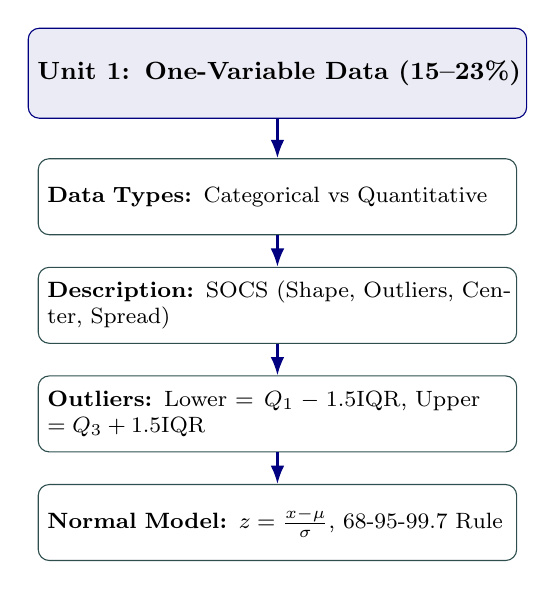
\begin{tikzpicture}[node distance=1.0cm, auto, >=Latex, 
    block/.style={rectangle, draw=NavyBlue, fill=NavyBlue!8, text width=2.4in, text centered, rounded corners, minimum height=0.45in, font=\small\bfseries},
    subblock/.style={rectangle, draw=DarkSlateGray, fill=white, text width=2.3in, rounded corners, minimum height=0.38in, font=\footnotesize}]
    
    \node [block] (root) {Unit 1: One-Variable Data (15--23\%)};
    \node [subblock, below=0.5cm of root] (data) {\textbf{Data Types:} Categorical vs Quantitative};
    \node [subblock, below=0.4cm of data] (socs) {\textbf{Description:} SOCS (Shape, Outliers, Center, Spread)};
    \node [subblock, below=0.4cm of socs] (outliers) {\textbf{Outliers:} Lower $= Q_1 - 1.5\text{IQR}$, Upper $= Q_3 + 1.5\text{IQR}$};
    \node [subblock, below=0.4cm of outliers] (norm) {\textbf{Normal Model:} $z = \frac{x-\mu}{\sigma}$, 68-95-99.7 Rule};

    \draw [->, thick, NavyBlue] (root) -- (data);
    \draw [->, thick, NavyBlue] (data) -- (socs);
    \draw [->, thick, NavyBlue] (socs) -- (outliers);
    \draw [->, thick, NavyBlue] (outliers) -- (norm);
\end{tikzpicture}%
}
\end{center}

\section{Essential Formulas \& Plain-English Translation}
\begin{formulabox}[Unit 1 Core Formulas]
\textbf{1. Sample Mean ($\bar{x}$):} $\bar{x} = \frac{\sum x_i}{n}$ --- The arithmetic average; non-resistant to skew/outliers.

\textbf{2. Sample Standard Deviation ($s_x$):} $s_x = \sqrt{\frac{\sum (x_i - \bar{x})^2}{n-1}}$ --- The typical distance of observations from the mean.

\textbf{3. Standardized Score ($z$-score):} $z = \frac{x - \mu}{\sigma}$ --- Number of standard deviations an observation falls above ($+$) or below ($-$) the mean.
\end{formulabox}

\section{Resistant vs. Non-Resistant Summary Statistics}
\begin{table}[H]
\centering
\adjustbox{max width=\linewidth}{%
\small
\begin{tabularx}{\linewidth}{@{}lXl@{}}
\toprule
\textbf{Measure} & \textbf{Resistant to Outliers / Skew?} & \textbf{When to Use on Exam} \\
\midrule
\textbf{Median \& IQR} & \textbf{Yes} (Middle 50\% only) & Skewed data or data with outliers \\
\textbf{Mean \& Standard Deviation} & \textbf{No} (Pulled toward the tail/extremes) & Symmetric, bell-shaped distributions \\
\bottomrule
\end{tabularx}%
}
\end{table}

\section{Top Exam Traps \& Sentence Frames}
\begin{trapbox}[Unit 1 Trap Alert: Comparative Language]
When comparing two distributions on an FRQ, you \textbf{must} use comparative words (\emph{"greater than", "less than"}). Stating two separate descriptions scores zero credit!
\end{trapbox}

\begin{templatebox}[Unit 1 FRQ Sentence Frame: $z$-Score Interpretation]
\emph{"The observed value of [context] is [z-score value] standard deviations [above/below] the mean of [context with units]."}
\end{templatebox}

% UNIT 2
\chapter{Unit 2: Exploring Two-Variable Data}

\section{Unit 2 Visual Mindmap}
\begin{center}
\adjustbox{max width=\linewidth}{%
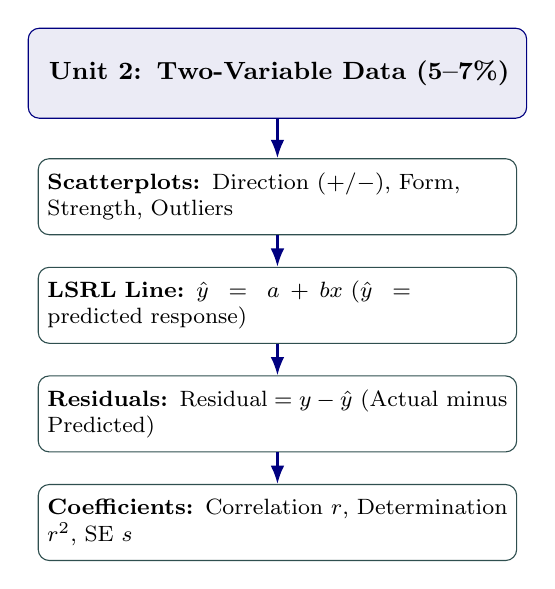
\begin{tikzpicture}[node distance=1.0cm, auto, >=Latex,
    block/.style={rectangle, draw=NavyBlue, fill=NavyBlue!8, text width=2.4in, text centered, rounded corners, minimum height=0.45in, font=\small\bfseries},
    subblock/.style={rectangle, draw=DarkSlateGray, fill=white, text width=2.3in, rounded corners, minimum height=0.38in, font=\footnotesize}]
    
    \node [block] (root) {Unit 2: Two-Variable Data (5--7\%)};
    \node [subblock, below=0.5cm of root] (scatter) {\textbf{Scatterplots:} Direction ($+/-$), Form, Strength, Outliers};
    \node [subblock, below=0.4cm of scatter] (lsrl) {\textbf{LSRL Line:} $\hat{y} = a + bx$ ($\hat{y} = \text{predicted response}$)};
    \node [subblock, below=0.4cm of lsrl] (res) {\textbf{Residuals:} $\text{Residual} = y - \hat{y}$ (Actual minus Predicted)};
    \node [subblock, below=0.4cm of res] (r2) {\textbf{Coefficients:} Correlation $r$, Determination $r^2$, SE $s$};

    \draw [->, thick, NavyBlue] (root) -- (scatter);
    \draw [->, thick, NavyBlue] (scatter) -- (lsrl);
    \draw [->, thick, NavyBlue] (lsrl) -- (res);
    \draw [->, thick, NavyBlue] (res) -- (r2);
\end{tikzpicture}%
}
\end{center}

\section{Essential Formulas \& Parameter Breakdowns}
\begin{formulabox}[Unit 2 Core Formulas: Linear Regression]
\textbf{1. Least-Squares Regression Line:} $\hat{y} = a + bx$ ($\hat{y} = \text{predicted response}$)

\textbf{2. Slope ($b$):} $b = r \left(\frac{s_y}{s_x}\right)$ --- Change in predicted $y$ per 1-unit increase in $x$.

\textbf{3. $y$-Intercept ($a$):} $a = \bar{y} - b\bar{x}$ --- The point $(\bar{x}, \bar{y})$ is always on the LSRL.

\textbf{4. Residual ($e$):} $\text{Residual} = y - \hat{y} = \text{Actual } y - \text{Predicted } \hat{y}$
\end{formulabox}

\section{Sentence Templates for FRQs}
\begin{templatebox}[Unit 2 FRQ Sentence Templates]
\textbf{1. Slope ($b$):} \emph{"For each additional 1 [unit of $x$], the predicted [response variable $y$] increases/decreases by approximately [value of $b$] [units of $y$]."}

\textbf{2. $r^2$:} \emph{"Approximately [value of $r^2 \times 100\%$] of the variation in [response variable in context] is accounted for by the linear model with [explanatory variable in context]."}

\textbf{3. Standard Error of Residuals ($s$):} \emph{"The typical distance between the actual [response variable $y$] and the predicted values from the regression line is approximately [$s$ units of $y$]."}
\end{templatebox}

% UNIT 3
\chapter{Unit 3: Collecting Data}

\section{Unit 3 Visual Flowchart: Sampling vs. Experimentation}
\begin{center}
\adjustbox{max width=\linewidth}{%
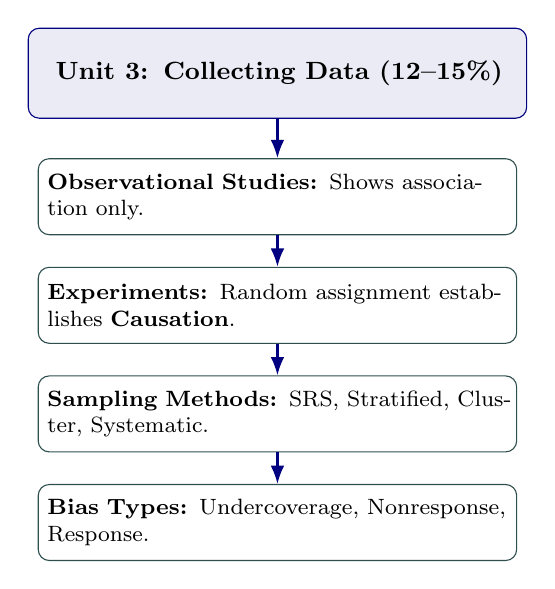
\begin{tikzpicture}[node distance=1.0cm, auto, >=Latex,
    block/.style={rectangle, draw=NavyBlue, fill=NavyBlue!8, text width=2.4in, text centered, rounded corners, minimum height=0.45in, font=\small\bfseries},
    subblock/.style={rectangle, draw=DarkSlateGray, fill=white, text width=2.3in, rounded corners, minimum height=0.38in, font=\footnotesize}]
    
    \node [block] (root) {Unit 3: Collecting Data (12--15\%)};
    \node [subblock, below=0.5cm of root] (obs) {\textbf{Observational Studies:} Shows association only.};
    \node [subblock, below=0.4cm of obs] (exp) {\textbf{Experiments:} Random assignment establishes \textbf{Causation}.};
    \node [subblock, below=0.4cm of exp] (sample) {\textbf{Sampling Methods:} SRS, Stratified, Cluster, Systematic.};
    \node [subblock, below=0.4cm of sample] (bias) {\textbf{Bias Types:} Undercoverage, Nonresponse, Response.};

    \draw [->, thick, NavyBlue] (root) -- (obs);
    \draw [->, thick, NavyBlue] (obs) -- (exp);
    \draw [->, thick, NavyBlue] (exp) -- (sample);
    \draw [->, thick, NavyBlue] (sample) -- (bias);
\end{tikzpicture}%
}
\end{center}

\section{The 4 Principles of Experimental Design}
\begin{enumerate}[leftmargin=*]
    \item \textbf{Comparison:} At least two treatment groups (or treatment vs. control) to isolate effects.
    \item \textbf{Random Assignment:} Balances the effects of confounding variables across treatment groups.
    \item \textbf{Control:} Keep all other outside variables constant.
    \item \textbf{Replication:} Apply treatments to sufficiently many experimental units.
\end{enumerate}

\begin{trapbox}[Unit 3 Trap Alert: Blocking vs. Stratification]
\textbf{Stratification} is used when \emph{sampling} from a population.\\
\textbf{Blocking} is used when \emph{assigning treatments} in an experiment.\\
Never mix these terms on an AP exam!
\end{trapbox}

% UNIT 4
\chapter{Unit 4: Probability, Random Variables, \& Distributions}

\section{Essential Formulas \& Probability Rules}
\begin{formulabox}[Unit 4 Core Formulas]
\textbf{1. Addition Rule:} $P(A \cup B) = P(A) + P(B) - P(A \cap B)$ (If disjoint, $P(A \cap B) = 0$).

\textbf{2. Conditional Probability:} $P(A \mid B) = \frac{P(A \cap B)}{P(B)}$

\textbf{3. Independence Test:} Events $A$ and $B$ are independent if $P(A \mid B) = P(A)$ or $P(A \cap B) = P(A) \cdot P(B)$.

\textbf{4. Combining Random Variables:}
$$\mu_{X \pm Y} = \mu_X \pm \mu_Y$$
$$\sigma_{X \pm Y}^2 = \sigma_X^2 + \sigma_Y^2 \quad \text{(\textbf{Always ADD variances!})}$$

\textbf{5. Binomial Distribution $B(n, p)$:}
$$P(X = k) = \binom{n}{k} p^k (1-p)^{n-k}$$
$$\mu_X = np, \qquad \sigma_X = \sqrt{np(1-p)}$$
\end{formulabox}

\begin{trapbox}[Unit 4 Trap Alert: Independence vs Disjoint]
Mutually exclusive (disjoint) events can \textbf{NEVER} be independent (if $P > 0$). Knowing $A$ happened means $B$ cannot happen!
\end{trapbox}

% UNIT 5
\chapter{Unit 5: Sampling Distributions}

\section{Unit 5 Core Formulas \& Central Limit Theorem}
\begin{formulabox}[Sampling Distributions]
\textbf{1. Sample Proportion ($\hat{p}$):}
$$\mu_{\hat{p}} = p, \qquad \sigma_{\hat{p}} = \sqrt{\frac{p(1-p)}{n}}$$
\emph{Normal if $np \ge 10$ and $n(1-p) \ge 10$.}

\textbf{2. Sample Mean ($\bar{x}$):}
$$\mu_{\bar{x}} = \mu, \qquad \sigma_{\bar{x}} = \frac{\sigma}{\sqrt{n}}$$
\emph{Normal if $n \ge 30$ by CLT or population is normal.}
\end{formulabox}

\begin{mnemonicbox}[Central Limit Theorem (CLT) Golden Rule]
The CLT states that the \textbf{sampling distribution of $\bar{x}$} becomes approximately normal as $n$ increases ($n \ge 30$), regardless of the shape of the underlying population! It does \emph{not} apply to individual observations.
\end{mnemonicbox}

% UNIT 6
\chapter{Unit 6: Inference for Proportions (Categorical Data)}

\section{1-Proportion vs. 2-Proportion Inference Procedures}
\begin{formulabox}[Unit 6 Formulas]
\textbf{1-Prop $z$-Interval:} $\hat{p} \pm z^* \sqrt{\frac{\hat{p}(1-\hat{p})}{n}}$

\textbf{1-Prop $z$-Test:} $z = \frac{\hat{p} - p_0}{\sqrt{\frac{p_0(1-p_0)}{n}}}$ (Use $p_0$ for Large Counts condition!)

\textbf{2-Prop $z$-Test (Pooled):}
$$\hat{p}_c = \frac{x_1 + x_2}{n_1 + n_2}$$
$$z = \frac{(\hat{p}_1 - \hat{p}_2) - 0}{\sqrt{\hat{p}_c(1-\hat{p}_c)\left(\frac{1}{n_1} + \frac{1}{n_2}\right)}}$$
\end{formulabox}

\begin{templatebox}[Unit 6 PANIC Template for 1-Prop $z$-Interval]
\textbf{P:} Let $p =$ true proportion of [context].\\
\textbf{A:} Random sample; $10\%$ condition ($n \le 0.10N$); Large counts ($n\hat{p} \ge 10, n(1-\hat{p}) \ge 10$).\\
\textbf{N:} 1-Proportion $z$-Interval.\\
\textbf{I:} Record $[ \text{Lower}, \text{Upper} ]$ with $95\%$ confidence.\\
\textbf{C:} \emph{"We are 95\% confident that the interval from [Lower] to [Upper] captures the true proportion of [context]."}
\end{templatebox}

% UNIT 7
\chapter{Unit 7: Inference for Means (Quantitative Data)}

\section{1-Sample $t$, Paired $t$, and 2-Sample $t$ Inference}
\begin{formulabox}[Unit 7 Means Formulas]
\textbf{1-Sample $t$-Interval:} $\bar{x} \pm t^* \left(\frac{s}{\sqrt{n}}\right) \quad (\text{df} = n - 1)$

\textbf{1-Sample $t$-Test:} $t = \frac{\bar{x} - \mu_0}{s / \sqrt{n}} \quad (\text{df} = n - 1)$

\textbf{2-Sample $t$-Test:} $t = \frac{(\bar{x}_1 - \bar{x}_2) - 0}{\sqrt{\frac{s_1^2}{n_1} + \frac{s_2^2}{n_2}}} \quad (\texttt{Pooled: NO})$
\end{formulabox}

\begin{trapbox}[Unit 7 Trap Alert: Paired $t$-Test vs. 2-Sample $t$-Test]
If data comes from pre/post tests, twins, or the same experimental unit measured twice, it is a \textbf{Paired $t$-Test} on the single list of differences ($L_1 - L_2$). Never run a 2-sample $t$-test on paired data!
\end{trapbox}

% UNIT 8
\chapter{Unit 8: Chi-Square Tests}

\section{The 3 Types of Chi-Square Tests}
\begin{table}[H]
\centering
\adjustbox{max width=\linewidth}{%
\small
\begin{tabularx}{\linewidth}{@{}lXXl@{}}
\toprule
\textbf{Test Name} & \textbf{Number of Samples} & \textbf{Variables} & \textbf{Degrees of Freedom} \\
\midrule
\textbf{$\chi^2$ Goodness of Fit} & 1 Sample & 1 Categorical Variable & $\text{df} = k - 1$ \\
\textbf{$\chi^2$ Homogeneity} & 2+ Independent Samples & 1 Categorical Variable & $\text{df} = (r-1)(c-1)$ \\
\textbf{$\chi^2$ Independence} & 1 Single Sample & 2 Categorical Variables & $\text{df} = (r-1)(c-1)$ \\
\bottomrule
\end{tabularx}%
}
\end{table}

\begin{formulabox}[Chi-Square Test Statistic]
$$\chi^2 = \sum \frac{(\text{Observed} - \text{Expected})^2}{\text{Expected}}$$
$$\text{Expected Count} = \frac{(\text{Row Total}) \times (\text{Column Total})}{\text{Table Total}}$$
\end{formulabox}

\begin{trapbox}[Unit 8 Condition Alert]
All \textbf{Expected Counts} must be $\ge 5$. Never check observed counts for this condition!
\end{trapbox}

% UNIT 9
\chapter{Unit 9: Inference for Slopes}

\section{Linear Regression Slope $t$-Test \& $t$-Interval}
\begin{formulabox}[Unit 9 Formulas]
\textbf{$t$-Interval for Slope $\beta$:} $b \pm t^* \cdot \text{SE}_b \quad (\text{df} = n - 2)$

\textbf{$t$-Test for Slope $\beta$:} $t = \frac{b - 0}{\text{SE}_b} \quad (\text{df} = n - 2)$
\end{formulabox}

\begin{mnemonicbox}[LINER Condition Checklist for Slopes]
\textbf{L} --- Linear pattern in scatterplot.\\
\textbf{I} --- Independent observations ($10\%$ rule).\\
\textbf{N} --- Normal distribution of residuals.\\
\textbf{E} --- Equal variance of residuals across line.\\
\textbf{R} --- Random sampling or assignment.
\end{mnemonicbox}

% CHAPTER 10: MASTER INFERENCE FLOWCHART
\chapter{Master Inference Selection Decision Flowchart}

\begin{table}[H]
\centering
\adjustbox{max width=\linewidth}{%
\small
\begin{tabularx}{\linewidth}{@{}lllXl@{}}
\toprule
\textbf{Data Type} & \textbf{Groups} & \textbf{Goal} & \textbf{Procedure Name} & \textbf{TI-84 Path} \\
\midrule
Categorical & 1 Sample & Estimate $p$ & \textbf{1-Prop $z$-Interval} & \texttt{STAT $\to$ TESTS $\to$ A} \\
Categorical & 1 Sample & Test $p$ & \textbf{1-Prop $z$-Test} & \texttt{STAT $\to$ TESTS $\to$ 5} \\
Categorical & 2 Samples & Estimate $p_1 - p_2$ & \textbf{2-Prop $z$-Interval} & \texttt{STAT $\to$ TESTS $\to$ B} \\
Categorical & 2 Samples & Test $p_1 = p_2$ & \textbf{2-Prop $z$-Test (Pooled)} & \texttt{STAT $\to$ TESTS $\to$ 6} \\
Categorical & 1 Sample (Fit) & Fit dist. & \textbf{$\chi^2$ GOF-Test} & \texttt{STAT $\to$ TESTS $\to$ D} \\
Categorical & 2+ Samples & Homogeneity & \textbf{$\chi^2$ Test of Homogeneity} & \texttt{STAT $\to$ TESTS $\to$ C} \\
Categorical & 1 Sample (2 Var) & Association & \textbf{$\chi^2$ Test of Independence} & \texttt{STAT $\to$ TESTS $\to$ C} \\
\midrule
Quantitative & 1 Sample & Estimate $\mu$ & \textbf{1-Sample $t$-Interval} & \texttt{STAT $\to$ TESTS $\to$ 8} \\
Quantitative & 1 Sample & Test $\mu$ & \textbf{1-Sample $t$-Test} & \texttt{STAT $\to$ TESTS $\to$ 2} \\
Quantitative & Matched Pairs & Difference $\mu_d$ & \textbf{Paired $t$-Test/Interval} & \texttt{T-Test on $L_1-L_2$} \\
Quantitative & 2 Indep Samples & Compare $\mu_1 - \mu_2$ & \textbf{2-Sample $t$-Test/Interval} & \texttt{STAT $\to$ TESTS $\to$ 4/0} \\
Quantitative & Linear Slope & Slope $\beta$ & \textbf{LinReg $t$-Test/Interval} & \texttt{STAT $\to$ TESTS $\to$ F/G} \\
\bottomrule
\end{tabularx}%
}
\end{table}

% CHAPTER 11: TOP 25 TRAPS
\chapter{Top 25 "Never-Forget" AP Grader Deduction Traps}

\begin{enumerate}[label=\textbf{\arabic*.}, leftmargin=*]
    \item \textbf{NEVER say "Accept $H_0$":} Always write \emph{"Fail to reject $H_0$"}.
    \item \textbf{NEVER write "We prove $H_a$":} Write \emph{"We have convincing statistical evidence for $H_a$"}.
    \item \textbf{Hypotheses in parameters ($\mu, p, \beta$), NEVER statistics ($\bar{x}, \hat{p}, b$).}
    \item \textbf{Always define parameters in context with units.}
    \item \textbf{Comparative language required on all distribution comparison FRQs (greater, lesser).}
    \item \textbf{Always put a hat ($\hat{y}$) on regression predicted values.}
    \item \textbf{Correlation ($r$) measures LINEAR strength only (never use $r$ for curved data).}
    \item \textbf{Association is NOT Causation.}
    \item \textbf{Blocking is for experiments; Stratification is for sampling.}
    \item \textbf{Mutually exclusive events are NEVER independent.}
    \item \textbf{Always ADD variances ($\sigma^2$), NEVER add standard deviations ($\sigma$).}
    \item \textbf{CLT applies to the sampling distribution of $\bar{x}$, not sample data.}
    \item \textbf{Use hypothesized $p_0$ for 1-Prop $z$-Test Large Counts ($np_0 \ge 10, n(1-p_0) \ge 10$).}
    \item \textbf{Use sample $\hat{p}$ for 1-Prop $z$-Interval Large Counts ($n\hat{p} \ge 10, n(1-\hat{p}) \ge 10$).}
    \item \textbf{Chi-square conditions require EXPECTED counts $\ge 5$, not observed counts.}
    \item \textbf{Chi-square df:} $\text{df} = (\text{rows}-1)(\text{cols}-1)$.
    \item \textbf{Never pool standard deviations for 2-sample $t$-tests (\texttt{Pooled: NO}).}
    \item \textbf{Confidence Interval (plausible values) vs Confidence Level (long-run capture rate).}
    \item \textbf{A high $r^2$ does NOT prove linearity (always check residual plot for random scatter).}
    \item \textbf{Voluntary response produces severe bias; results cannot be generalized.}
    \item \textbf{State test conclusion in terms of $H_a$ in context.}
    \item \textbf{State the significance level ($\alpha$) explicitly in decision sentences.}
    \item \textbf{Calculator Speak alone scores ZERO on FRQs (must write formulas and parameter names).}
    \item \textbf{Extrapolation is dangerous (do not predict $\hat{y}$ outside the domain of $x$).}
    \item \textbf{Context, Context, Context: Include problem units and scenario in every sentence!}
\end{enumerate}

% CHAPTER 12: SENTENCE FRAME DIRECTORY
\chapter{Standard FRQ Interpretation Sentence Frames}

\begin{templatebox}[Frame 1: Confidence Interval for a Parameter]
\emph{"We are [C\%] confident that the interval from [Lower] to [Upper] captures the true [proportion / mean] of [context with units]."}
\end{templatebox}

\begin{templatebox}[Frame 2: Confidence Level ($C\%$)]
\emph{"If we take many random samples of the same size and construct [C\%] confidence intervals, about [C\%] of the intervals will capture the true [parameter in context]."}
\end{templatebox}

\begin{templatebox}[Frame 3: $p$-Value in Context]
\emph{"Assuming that [null hypothesis $H_0$ in context] is true, there is a [p-value] probability of obtaining a sample statistic as extreme as or more extreme than observed, purely by random chance."}
\end{templatebox}

\begin{templatebox}[Frame 4: Reject $H_0$ Conclusion]
\emph{"Because the $p$-value ($[p]$) is less than $\alpha$ ($[0.05]$), we reject $H_0$. There is convincing statistical evidence that [state $H_a$ in context]."}
\end{templatebox}

\begin{templatebox}[Frame 5: Fail to Reject $H_0$ Conclusion]
\emph{"Because the $p$-value ($[p]$) is greater than $\alpha$ ($[0.05]$), we fail to reject $H_0$. There is NOT convincing statistical evidence that [state $H_a$ in context]."}
\end{templatebox}

\end{document}
